\chapter{Beasts of Prey or Rational Animals? Private Governance in Brazil's \emph{Jogo do Bicho}}
\label{chap:bicho}

\section{Introduction}
\label{sec:intro}

In 1892, Baron João Batista de Viana Drummond came up with a new idea to fund his cash-strapped zoo. Situated in a quiet neighbourhood in the north of Rio de Janeiro, the \emph{Jardim Zoológico,} or Zoological Garden, hosted a variety of exotic species and offered breath-taking views of the city. But it lacked visitors. As an experienced businessman, Drummond soon realised the zoo would have to provide other kinds of entertainment to keep itself afloat. Among his suggestions, one seemed particularly promising: a lottery raffle.

The rules were straightforward. In the morning, the Baron would choose one animal from a list of 25 beasts and put its picture inside a wooden box at the zoo's entrance. Visitors who wanted to join the raffle received a ticket bearing the stamp of one of those 25 animals.\footnote{At first, the zoo staff distributed the tickets at random, making the game similar to a common raffle. But it did not take long until visitors could name their animals of choice. This change made the game considerably more appealing and lasts until this day \citep[71--74]{da1999aguias}.} At five in the afternoon, Drummond opened the box, showed the picture to the public, and paid to every winner a cash prize worth 20 times the zoo's admission fee.\footnote{The amount was higher than a carpenter's monthly wage \citep[542]{chazkel2007beyond}.} The lottery was labelled as the \emph{jogo do bicho}, or the animal game, and it was immediately adopted by the public. Eager to capitalise on that initial success, Drummond stated that visitors could buy tickets not only at the zoo, but in stores across Rio de Janeiro. He rightly predicted that this small change would increase profits, but there was one thing the Baron did not foresee. He unleashed a new gambling market.

The \emph{jogo do bicho} craze swept the whole city after independent sellers entered the marketplace \citep{magalhaes2005ganhou, soares1993jogo}. A network of street bookmakers, called \emph{bicheiros}, expanded spontaneously the original game in innovative ways. Evading state regulations, \emph{bicheiros} made the lottery available in every part of Rio by scalping tickets or promoting their own versions of the clandestine numbers game  \citep[37]{chazkel2011laws}. The \emph{jogo do bicho} became so widespread that Olavo Bilac, a major literary figure in nineteenth-century Brazil, summarised the situation as follows: `Today {[}1895{]}, in Rio de Janeiro, the game is everything. {[}\ldots{}{]} Nobody works! Everybody plays' \citep[43]{pacheco1957antologia}.\footnote{Unless otherwise noted, all translations from the Portuguese are my own.} But this tolerant state of affairs did not last. Civil servants and police officers criminalised the \emph{jogo do bicho} on the grounds of `public safety', and in the late 1890s they launched a country-wide campaign against the lottery \citep{benatte2002jogos, krelling2014jogos, villar2008contravencao}.\footnote{The National Lottery Company (\emph{Companhia das Loterias Nacionaes do Brazil}), a public-private partnership founded four years after the creation of the \emph{jogo do bicho}, also lobbied actively for a hard-line stance against the \emph{bicheiros} \citep[82]{da1999aguias}.}

Yet the game has survived. The animal game has outlasted more than 30 Brazilian presidents and thrived under military regimes and democratic governments alike \citep{gaspari2002ditadura, jupiara2015poroes}. But more than a act of defiance, the \emph{jogo do bicho} is a successful capitalist enterprise \citep{labronici2014sorteio, magalhaes2005ganhou}. A recent study by Fundação Getúlio Vargas, a Brazilian think tank, affirmed that the \emph{jogo do bicho} earns from BRL 1.3 to BRL 2.8 billion per year (USD 400 to USD 850 million), making it the largest clandestine gambling game in the world.\footnote{See \url{http://goo.gl/9kNeX8} and \url{http://goo.gl/8FSAZl} (in Portuguese). Access: December 2016.} \citet[171]{schneider1996brazil} estimated that in the 1990s, the game furnished about 50,000 jobs in the Rio de Janeiro city alone, almost the same number of employees that the oil giant Petrobras had in 2011 \citep{exame2013petrobras}.\footnote{In 1966, Time Magazine wrote that the \emph{jogo do bicho} was `the largest single industry in Latin America' and employed about 1\% of the Brazilian workforce. See \url{http://content.time.com/time/magazine/article/0,9171,842527-1,00.html}. Access: December 2016.}

\begin{figure}[!htbp]
	\centering
	\begin{minipage}[b]{0.45\textwidth}
		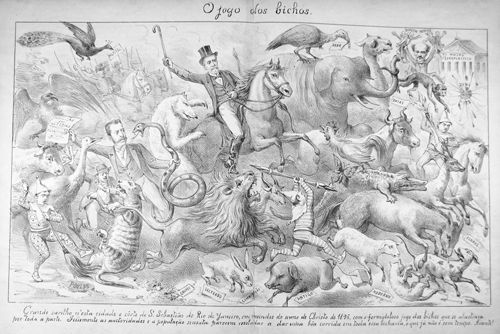
\includegraphics[width=\textwidth, height=6cm]{images/bicho01.jpg}
	\end{minipage}
	\hfill
	\begin{minipage}[b]{0.45\textwidth}
		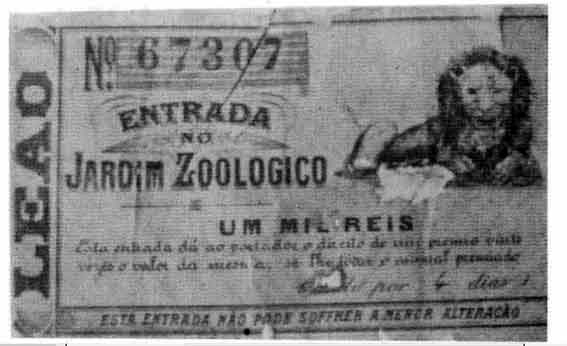
\includegraphics[width=\textwidth, height=6cm]{images/bicho02.jpg}
	\end{minipage}
	\caption{Left: cartoon of the Baron of Drummond and the animals of the \emph{jogo do bicho} (1896). Right: entry ticket to Rio's Zoological Garden that allowed the bearer to join the raffle. Sources: Instituto Histórico e Geográfico Brasileiro, Rio de Janeiro, Revista Illustrada, ano 21, no. 718 (1896) and Museu da Imagem e do Som, Rio de Janeiro. Reproduced in \citet[35--36]{chazkel2011laws}.}
	\label{fig:barao}
\end{figure}

Moreover, the animal game plays a crucial role in the expansion of Rio de Janeiro's Carnival Parade, a popular festivity synonymous with Brazil at home and abroad \citep{araujo2003carnaval,costa2001100,da1973carnaval, da1979carnavais,vianna1995misterio}. \emph{Bicheiros} donate hefty sums to `samba schools' to gather support of poor communities and, no less importantly, to co-opt local politicians attracted by the financial and electoral gains offered by the festival \citep{cavalcanti2006carnaval, queiroz1992carnaval}. This patron-client relationship has been proven effective: in 2016, the Carnival generated about USD 900 million in revenue and the Rio de Janeiro state received more than one million tourists.\footnote{Data provided by the Brazilian government. See \url{https://goo.gl/XMcbTM} (in Portuguese). Access: December 2016.}

In this article I offer a rational choice interpretation of the \emph{jogo do bicho} and discuss how \emph{bicheiros} promote social order, solve information asymmetries, and reduce negative externalities. My analysis discusses three strands of academic literature. First, this work contributes to the scholarship on extra-legal institutions, mainly to the literature on collective action within criminal organisations. For instance, \citet{gambetta1996sicilian} examines the strategies used by the Sicilian Mafia to settle disputes among their members and enforce rules in the areas they exercise control. \citet{leeson2007arrgh,leeson2009invisible,leeson2010pirational} affirms that pirate groups employed hard-to-fake signals to increase the profitability of their operations. \citet{skarbek2011governance,skarbek2012prison,skarbek2014social}, in turn, highlights the role of written and implicit norms in mitigating rent-seeking and coordinating productive activities in California prison gangs. I argue that \emph{bicheiros} have employed reputation strategies and provided club goods to enforce private contracts and foster trust among criminals. Moreover, I also describe how \emph{bicheiros} have developed sophisticated financial mechanisms, such as informal hedging operations and risk-sharing contracts, to prevent predatory behaviour in their community.

Second, this work relates to the literature on repugnant transactions and the relationship between morality and the market \citep{boettke1995morality, roth2007repugnance, sandel2012money, satz2010some, simmel1900geldes, zelizer1979morals}. In the following sections, I claim that the Brazilian elites have attached pejorative meaning to the \emph{jogo do bicho} to constrain the gambling market. I provide evidence that \emph{bicheiros} were aware of this problem, and as a response, they devised a series of rules aimed at reducing the costs associated with repugnance \citep{labronici2014sorteio, magalhaes2005ganhou}. \emph{Bicheiros} have made considerable efforts to increase the levels of trust in the system and distance themselves from other types of illegal activities. Their main tool to increase credibility was costly signalling, that is, the \emph{bicheiros} hoped the public would see them as credible brokers by sacrificing their immediate interests  \citep{gambetta2009codes,kimbrough2015commitment, schelling1960strategy}.

Lastly, this work connects to the literature on state capture, which is among the most important topics in public choice theory \citep{hellman2003seize, rose1978corruption, rose1999corruption, shleifer2002grabbing, tollison1982rent}. More specifically, I use the Brazilian case to illustrate how politicians and civil servants can be co-opted by criminal groups and produce sub-optimal social outcomes. \citet{queiroz1992carnaval} explored why \emph{bicheiros} turned into patrons of the Carnival's samba schools and affirmed that this influence gave them leverage over political authorities. \citet{misse2007illegal} investigated the links between bicheiros and police officers, and suggested that the illegal lottery had been the main cause of police corruption in Rio de Janeiro until the 1970s. In a similar vein, \citet{jupiara2015poroes} analyse the relationship between the \emph{jogo do bicho} and the military regime in Brazil (1964--1985). I supplement this literature by highlighting how asymmetrical information, agency dilemmas, and rent-seeking behaviour offer convincing explanations to the issues presented above. Although those concepts have a long tradition in public choice, scholars have not applied those ideas thus far to understand the dynamics of the \emph{jogo do bicho}. By doing so, I integrate seemingly contradictory historical facts into a single narrative that connects micro-level decisions to macro-level outcomes.

The remainder of this article proceeds as follows. Section \ref{sec:organisation} presents a brief historical overview of the \emph{jogo do bicho}. It describes the necessary conditions for the emergence of the game and presents its basic organisational structure. Section \ref{sec:governance} details the \emph{jogo do bicho}'s governance mechanisms, particularly the strategies employed by vendors to increase trust in markets that operate at the margins of the law. Section \ref{sec:capture} discusses the links between illegal gambling markets, samba schools and the Brazilian state. Section \ref{sec:conclusion} offers some concluding remarks.

\section{\emph{Jogo do Bicho} as an Emergent Institution}
\label{sec:organisation}

\subsection{Historical Background}
\label{sub:background}

The early history of the \emph{jogo do bicho} is a textbook example of spontaneous order. Spontaneous orders are emergent macro-level phenomena that result from voluntary actions of purposive, self-interested individuals utilising their contextual knowledge \citep{boettke1990theory, boettke2005methodological, hayek1945use, hayek1960constitution, hayek1973law, leeson2008coordination, menger1871grundsatze, polanyi1948planning, polanyi1951logic}. Drummond, the Zoological Garden's original owner, designed the basic framework for the \emph{jogo do bicho}; but independent bookmakers were the ones who popularised the game \citep[77]{magalhaes2005ganhou}. Ticket sellers could quickly respond to market signals and then allocate their products where they were more valuable because of the lack of central coordination. Moreover, competition among sellers fostered innovation, and the \emph{bicheiros} invented new game rules to make the lottery more appealing to their customers \citep[61]{mello1989historia}. In this sense, the animal game is the materialisation of an evolutionary process of entrepreneurial discovery in which the interactions that provided the highest value to consumers were preserved over time \citep{boettke2008gordon, boettke2014entrepreneurship, buchanan1964should, hayek1978competition, kirzner1997entrepreneurial}.

However, the \emph{jogo do bicho} only emerged because of historically contingent circumstances. The late nineteenth-century Brazil had four characteristics that explain how the animal game came to being: 1) a growing urban population excluded from the formal labour market; 2) an inflow of immigrants whose extended family networks helped them engage in trade; 3) an expansion of the monetary supply in the first years of the republic (1880s--1890s); and 4) a judicial system that, albeit repressive, had only imperfect law enforcement. Figure \ref{fig:dag} presents a simple directed acyclic graph (DAG) \citep{pearl2009causality} that shows the relationships between these explanatory variables and the development of the \emph{jogo do bicho}.\footnote{The main purpose of direct acyclic graphs is to graphically display the possible links among the exposure variables, confounders, and outcomes \citep{morgan2014counterfactuals, pearl2009causality}. DAGs are transparent by definition, as all theoretical choices made by the researcher are stated explicitly in the model. Each single-headed arrow in a DAG indicates that the variable at the origin causes the variable at the end of the directed edge. Dashed edges suggest that two variables are jointly dependent on unobserved common causes. There are no assumptions regarding the functional form of the relationships, and unless mentioned otherwise, the arrows represent fully non-parametric associations. Variables between two nodes are mediators, and variables pointed at by two or more factors have multiple causes. They are called \emph{colliders}. For the sake of clarity, errors are assumed independent and often excluded from the graphs. For an accessible introduction to DAGs see \citet[chap. 3--4]{morgan2014counterfactuals} and \citet{pearl2016causal}.}

\begin{figure}[!htbp]
	\begin{tikzpicture}[->,>=stealth',shorten >=4pt,auto,node distance=3cm, semithick][h]
		% nodes %
		\node[circle,fill,inner sep=3pt,label=above right: \shortstack{Urban \\ Poverty}] (p) {};
		\node[circle,fill,inner sep=3pt,label=right: \shortstack{Jogo \\ do Bicho}, right = 8 of p] (y) {};
		\node[circle,fill,inner sep=3pt,label=below left: {Immigration}, below = 3 of p] (i) {};
		\node[circle,fill,inner sep=3pt,label=above:{Money Supply}, above = 3 of p] (m) {};
		\node[circle,fill,inner sep=3pt,label=below right:{Social Ties}, right = 3 of i] (s) {};
		\node[circle,fill,inner sep=3pt,label=above:{Weak Law Enforcement}, above = 3 of y] (l) {};
		\node[circle,fill=white, draw, outer sep=0pt, inner sep=3pt,label= left: \shortstack{Correlated \\ Background Factors}, above left = 2 of p] (u) {};
		% edges %
		\draw[->, line width = 1.2] (p) -- (y);
		\draw[->, line width = 1] (s) -- (y);
		\draw[->, line width = 1] (i) -- (s);
		\draw[->, line width = 1.2] (l) -- (y);
		\draw[->, line width = 1] (m) -- (y);
		\draw[->, line width = 1.2] (i) -- (p);
		\draw[->, dashed, line width = 1] (u) -- (p);
		\draw[->, dashed, line width = 1] (u) -- (m);
	\end{tikzpicture}
	\caption{Directed Acyclic Graph -- Explanatory Variables for the \emph{Jogo do Bicho}}
	\label{fig:dag}
\end{figure}

I start with the impact of urban poverty on the animal game. Brazil abolished slavery in the late 1880s, a period in which the country was rapidly urbanising and freed slaves migrated to its growing cities \citep{andrews1991blacks, fausto2014concise, naro1992revision, skidmore1993black}. The former slaves were joined by increasing numbers of Asian and European immigrants \citep{hall1969origins, lesser2013immigration, smith1979ethnic}. Nevertheless, the job market tightened considerably after the \emph{Encilhamento} financial crisis of 1891 \citep{topik2014political, triner2005baring}. During the economic downturn, the informal economy was an obvious destination for the urban poor. Given its widespread popularity, the \emph{jogo do bicho} attracted hopeful entrepreneurs, either Brazilian or foreign-born, who could not enter the formal labour force.\footnote{The underground economy was also more democratic than the formal sector. As \citet[115]{chazkel2011laws} observes, one of the few professions open to poor women and foreigners in the early 1900s was that of street vendor. These vendors used to sell different types of merchandise and many of them would later offer \emph{jogo do bicho} tickets.}

The immigration also influenced the \emph{jogo do bicho} via social ties. Most foreigners who moved to Brazil came from countries, such as Portugal, Spain or Italy, where extended families were the basic form of social organisation \citep{klein1994imigraccao, lobo2001imigraccao, trento1989outro}. Family and neighbourhood networks created incentives for immigrants to establish trade relations and enforce cooperation through community responsibility systems \citep{roth2014prison}. Because of these particular social characteristics, in the 1890s foreigners were over-represented in the Brazilian trade in general \citep{mattos1991vadios, oliveira2001brasil, truzzi2008patricios} and in the \emph{jogo do bicho} in particular \citep{godoi2012imigraccao, magalhaes2005ganhou, torcato2011repressao, villar2008contravencao}. Although kinship bonds became less relevant over time, these links offered an important element of social cohesion in the \emph{jogo do bicho}'s formative years.

Next is the impact of expanded monetary supply. The abolition of slavery and the growing industrialisation of Brazil increased the amount of capital available in the country \citep{franco1987reformas, schulz2008financial}. The 1888 Banking Act gave extra liquidity to local financial markets, and the \emph{jogo do bicho} entrepreneurs utilised that increase in the monetary base to extend the scope of their business. Some years later, the animal game would be available not only across the city of Rio de Janeiro but throughout Brazil \citep[76]{da1999aguias}.

The country's lax financial policy might correlate with poverty through unspecified factors. For instance, political decisions may have caused inadvertently both poverty and the expansion of the monetary base \citep{mattos2013shantytown, schmidt1982modernization}; alternatively, external events such as institutional instability \citep{costantini2014index, fausto2014concise, luna2014economic} or commodity shocks \citep{musacchio2014colonial} could be the cause of those two variables. There is not enough evidence to discard such scenarios. To illustrate this uncertainty, the two nodes, namely, money supply and urban poverty, are connected with a dashed edge in Figure \ref{fig:dag}.

The last necessary condition for the emergence of the \emph{jogo do bicho} is weak law enforcement. \citet[69--100]{chazkel2011laws} notes that until the 1940s police district chiefs operated within a large margin of discretion and repression against bookmakers was idiosyncratic. Prosecution against the \emph{bicheiros} had hardened in 1917, but only in 1946, when the federal government banned all gambling activities in the country \citep[155--156]{magalhaes2005ganhou}, the law was consistently enforced.

\subsection{Organisational Structure}
\label{sub:organisation}

The animal game has three levels of hierarchy. At the bottom are the \emph{bicheiros}, who are those in charge of selling \emph{jogo do bicho} tickets \citep{chazkel2007beyond, chazkel2011laws, da1999aguias, labronici2014sorteio, magalhaes2005ganhou, misse2007illegal}. \emph{Bicheiros} are the most visible part of the \emph{jogo do bicho} structure. The bookmakers often build their vending stands inside the premises of a local shop, such as a small grocery store or a pub, and are recognisable by their chairs facing the street, stamps and blocks of paper \citep[259]{chazkel2011laws}. \emph{Bicheiros} usually work alone, but they may employ up to 10 people depending on how busy their betting site is \citep[69]{labronici2014sorteio}.

The \emph{gerentes} (managers) oversee all \emph{jogo do bicho} stands in a given area. Their task is akin to that of a firm accountant. Gerentes control the cash flow between the \emph{bicheiros} and the bankers, manage the payroll of the employees, and provide financial information to the top members of the organisation. They also supervise individuals who carry menial tasks in the business, transfer money to other gambling branches and double-check the balance sheets of the betting sites \citetext{\citealp[71]{labronici2012paratodos}; \citealp[142]{misse2007illegal}}.

\begin{figure}[!htbp]
	\centering
	\begin{minipage}[b]{0.45\textwidth}
		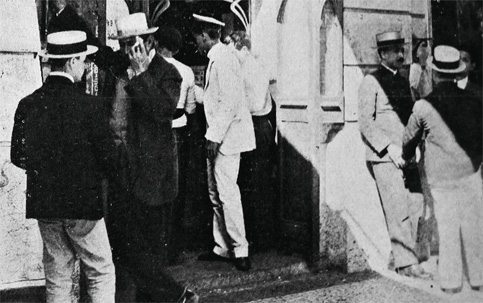
\includegraphics[width=\textwidth, height=6cm]{images/bicho03.jpg}
	\end{minipage}
	\hfill
	\begin{minipage}[b]{0.45\textwidth}
		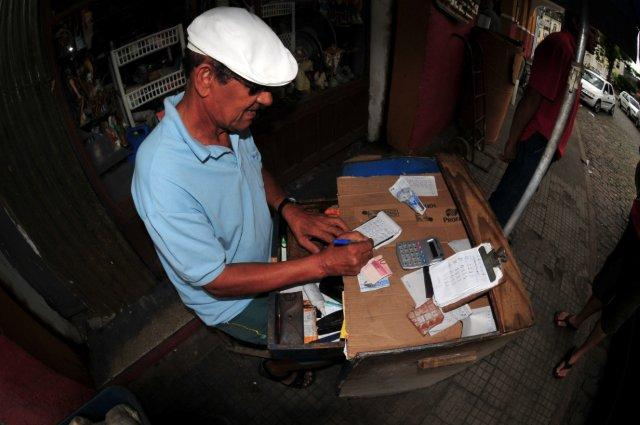
\includegraphics[width=\textwidth, height=6cm]{images/bicho04.jpg}
	\end{minipage}
	\caption{\emph{Jogo do bicho} betting sites in 1917 and in 2011. The picture on the right shows a \emph{bicheiro}, a street-corner vendor. Sources: \citet{alecrim2012bicho} and \citet{ferrarini2011bicho}.}
	\label{fig:banca1917}
\end{figure}

The \emph{banqueiros}, or the Portuguese for bankers, occupy the top position in the \emph{jogo do bicho} hierarchy, comprising the small financial elite of the game. A 2012 report by the Brazilian Federal Police affirmed that 10 \emph{banqueiros} controlled the market throughout the country; five of them based in the state of Rio de Janeiro \citep{globo2012contraventores}. Apart from funding the game, the bankers provide support for the employees to undertake their activities. The \emph{banqueiros}' main attributions include paying bribes to police personnel, bailing out sellers arrested by security forces, and offering judicial assistance to employees in case of legal persecution \citep[75]{labronici2012paratodos}.

\emph{Banqueiros} run their businesses from fortified houses in unknown locations, the \emph{fortalezas} (`forts'). The first \emph{fortalezas} likely appeared in the 1950s, when the animal game was already well-established across the Brazilian territory. The period coincides with a time when the \emph{jogo do bicho} finances had become increasingly concentrated in fewer hands \citep[259]{chazkel2011laws}. Due to the growing size of the \emph{jogo do bicho} economy, \emph{banqueiros} decided to move their operations away from the public to avoid police persecution and reduce coordination costs.

Although the forts provided safety to the bankers, the existence of those hideouts posed a challenge to the organisation. Bankers removed from the public view are not accountable to players and booking agents. Similarly, bankers and managers working in the \emph{fortalezas} cannot oversee their employees as effectively as before. Considering that the animal game itself is illegal and the amount of money involved in the bets is often substantial, both \emph{banqueiros} and booking agents have strong incentives to defect. Players, in turn, have no evident reason to trust \emph{banqueiros} or \emph{bicheiros}. How do \emph{jogo do bicho} agents overcome trust issues and cooperate under uncertainty?

I argue that the \emph{jogo do bicho} solves problems of internal cooperation by providing club goods \citep{buchanan1965economic, berman2008religion, berman2009radical, leeson2011government, roth2014prison} while simultaneously shunning cheaters through punishments and appeals to `the shadow of the future' \citep{axelrod1984evolution, axelrod1985achieving, bo2005cooperation, roth1978equilibrium}. Clients and \emph{bicheiros} cooperate based on trust-enhancing mechanisms, most of them devised specifically for the \emph{jogo do bicho} \citep{da1999aguias, magalhaes2005ganhou}. Such mechanisms are relevant because they have allowed the \emph{jogo do bicho} to distance itself from other shadow markets and become a profitable enterprise in the long run.

\section{Governance of the \emph{Jogo do Bicho}}
\label{sec:governance}

\subsection{Gambling Markets and Repugnant Transactions}
\label{sub:repugnance}

The \emph{jogo do bicho} is a repugnant market. Individuals that like to gamble cannot do so because of strong moral objections from outsiders \citep{brisset2016marche, roth2007repugnance, satz2010some, zelizer1979morals}. As early as in 1890, Brazilian public authorities positioned themselves against the \emph{jogo do bicho} arguing that `{[}\ldots{}{]} this type of amusement is prejudicial to the interests of the unwise, who are naively seduced by the deceptive hope of uncertain lucre' \citep[544]{chazkel2007beyond}. In 1941, the government banned the animal game;\footnote{See: \url{http://www.planalto.gov.br/ccivil_03/decreto-lei/Del3688.htm} (in Portuguese). Access: December 2016.} five years later, it prohibited all games of chance.\footnote{The 1946 decree stated that gambling was `harmful to morality and the good customs', hence `[\dots] the repression against games of chance [was] an imperative of the universal consciousness'. The text can be read at: \url{http://www.planalto.gov.br/ccivil_03/decreto-lei/Del9215.htm} (in Portuguese). Access: December 2016.} The \emph{jogo do bicho}, casinos and bingos remain illegal in the country. Recent estimations show that the prohibition of the \emph{jogo do bicho} have prevented the state from earning BRL 15 to BRL 20 billion (USD 4.5 to USD 6 billion) per year in expected taxation revenues, aside from the subjective utility losses for players. \citep{congressoemfoco2015bicho, fsp2016legalizarbicho}.

In contrast with the official statements, the noxious element of the \emph{jogo do bicho} does not come from its inherent randomness. The game is `repugnant' precisely because it is \emph{a market}, a setting in which individuals can monetise the entertainment for private profit \citep{chazkel2007beyond, chazkel2011laws}. The Brazilian state has never seen any contradiction between banning games of chance and running a national lottery company of its own; even the Catholic Church, which has long condemned the \emph{jogo do bicho}, frequently organises raffles to fund its activities \citep[49]{abreu1996imperio, magalhaes2005ganhou}. Only after the introduction of private money that Brazilians objected the idea of benefiting from someone else's bad luck.

In this sense, the main obstacle that confronted \emph{bicheiros} was to convince others that the animal game would not cause the Brazilian society `to slide down a slippery slope to genuinely repugnant transactions' \citep[45]{roth2007repugnance} such as prostitution or debt bondage. As the century-old history of the game can attest, \emph{bicheiros} have succeeded in this task. But how? The literature on repugnant costs tell us little about how markets transition from noxious to tolerated. Here I posit two mechanisms that reduced the stigma associated with the game: 1) \emph{a strong reputation of honesty} expressed by costly signals from sellers, and 2) the provision of \emph{selective incentives} for both clients and booking agents. Below, I offer evidence that these two factors allowed the animal game to reach its current semi-legal status in Brazil.

\subsection{External Cooperation}
\label{sub:external}

Evolutionary game theory \citep{axelrod1984evolution, axelrod1985achieving, smith1982evolution} and experimental studies \citep{dawes1977behavior, isaac1984divergent, kim1984free, marwell1981economists} have both demonstrated that long-term cooperation is possible whenever players expect future pay-offs to be higher than present ones. Fear of retaliation induces individuals not to cheat. Nevertheless, illegal organisations tend to discount the future even more heavily than the other groups, what makes cooperative behaviour among criminals uncommon \citep{gambetta2009codes, skarbek2011governance,skarbek2012prison,skarbek2014social}. The \emph{jogo do bicho} is an exception to this rule. The market properties of the game and inconsistent repression by Brazilian authorities have permitted \emph{bicheiros} to overcome the stigma of repugnance and improve the game's long-term profitability.

The \emph{jogo do bicho} entrepreneurs have made considerable efforts to present themselves as honest brokers. The first trust-enhancing mechanism they have employed to foster external cooperation was the use of a \emph{fixed-multiplier formula} for pay-outs. It works as follows. If a player wins the lowest prize of the animal game, he or she receives 18 times his/her investment regardless of the size of the bet. Bigger prizes naturally offer higher returns; a lucky winner of the top prize wins up to 4,000 times the value of his/her bet \citetext{\citealp[89]{labronici2012paratodos}; \citealp[20]{magalhaes2005ganhou}}.

This stands in sharp contrast to the common practice of sharing a prize among winners. Lottery pay-outs demand high levels of interpersonal trust: players rely on unverifiable information about the total funds collected by the lottery, and they can never be sure whether the payments are evenly distributed. The fixed-multiplier formula alleviates such problems of adverse selection \citep{akerlof1970market, cohen2010testing, levin2001information}. As players and vendors known the prize value beforehand, the method provides consumers with complete information about their individual prizes while also binding the \emph{bicheiros} to a contract that can be easily enforced. This technique offers buyers a simple yet effective screening strategy that induces \emph{bicheiros} to provide honest information about the game \citep{spence1973job, stiglitz1981credit}.

\emph{Bicheiros} have addressed information asymmetries in another ways. Since the 1950s, when the \emph{jogo do bicho} bankers had moved their operations to the \emph{fortalezas}, the public could not oversee the lottery draws \citep[259]{chazkel2011laws}. This could lead to a decline in trust among buyers and vendors of lottery tickets and, as a result, to reduced profits. \emph{Bicheiros} have mitigated this problem with a two-pronged strategy. First, they started to utilise the winning numbers from the licit government-run lottery, the \emph{Loteria Federal}, instead of their own draws \citetext{\citealp[546]{chazkel2007beyond}; \citealp[89]{labronici2012paratodos}; \citealp[39-40]{mello1989historia}}. The federal lottery numbers are public information. The media broadcasts the draws on radio and TV, so any interested player can verify the selected numbers. The Loteria Federal is also audited by two independent state institutions, a private accounting firm, and voluntary members of the public; hence, \emph{bicheiros} can free ride on the lottery's long-standing reputation of credibility.\footnote{As of April 2016, the lottery was audited by the \emph{Controladoria Geral da União} (Comptroller General of Brazil), the \emph{Tribunal de Contas da União} (General Accounting Office), and by Ernst \& Young. The balls are measured and weighted every three months by the National Institute of Metrology, Quality and Technology (Inmetro), the Brazilian equivalent of United Kingdom's National Physical Laboratory or the American National Standards Institute. See \url{http://noticias.uol.com.br/cotidiano/ultimas-noticias/2016/04/08/auditoria-dos-sorteios-da-caixa-e-confiavel-veja-como-e-o-processo.htm} (in Portuguese). Access: December 2016.}

\begin{figure}[!htbp]
	\centering
	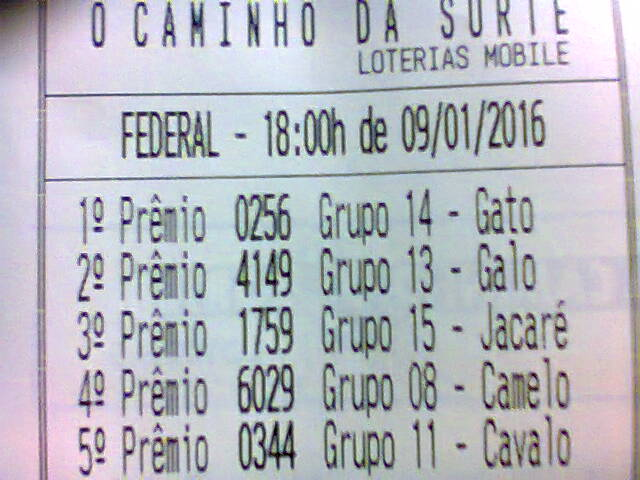
\includegraphics[width=\textwidth, height=6cm]{images/bicho06.jpg}
	\caption{Results of a \emph{jogo do bicho} draw from 09 January 2016. `Federal' means that the winning numbers were drawn by the federal government lottery. The first prize was group 14, the cat. Source: Unknown. Available at: \url{https://goo.gl/6PHV8u}. Access: December 2016.}
	\label{fig:federal}
\end{figure}

Second, they included representatives of all major \emph{jogo do bicho} bankers in every draw and independently publicise the game results. Certain \emph{bicheiros} went as far as publishing the numbers in Rio's newspapers. In the early twentieth century, some tabloids were entirely dedicated to the game \citep[60]{magalhaes2005ganhou}. Booking agents see this strategy as a credible signal from the game financiers, as providing contrasting information would indicate game manipulation. Moreover, collusion can also be spotted if the draws show repeated numbers or unusual patterns.

\begin{figure}[!htbp]
	\centering
	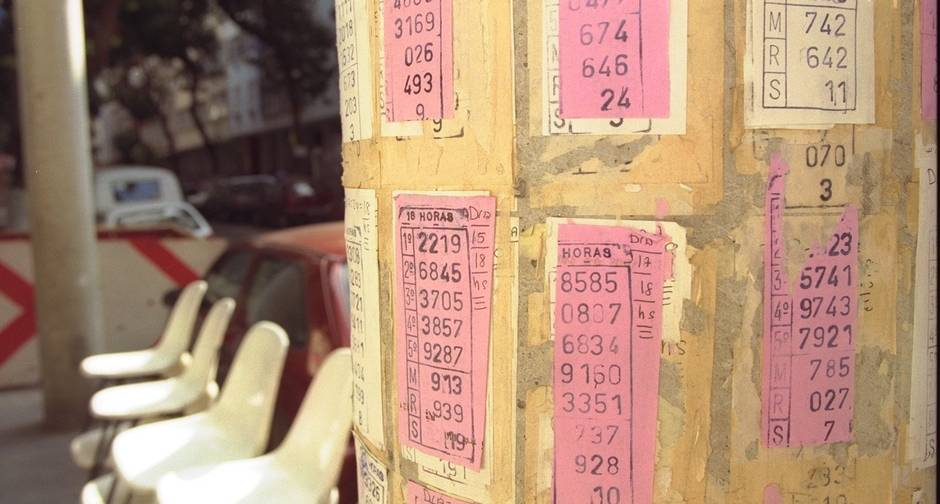
\includegraphics[width=\textwidth, height=6cm]{images/bicho05.jpg}
	\caption{\emph{Jogo do bicho} results are fixed on light poles in Rio de Janeiro. Source: \citet{gomes1998bicho}.}
	\label{fig:poste}
\end{figure}

These efforts have proved popular with the game enthusiasts. One often-repeated saying about the \emph{jogo do bicho} is that `in the \emph{jogo do bicho}, what is written down counts' \citep[159]{chazkel2011laws}, that is, buyers and sellers do fulfill their informal obligations without third-party enforcement. Such mutual confidence reduces the potential for conflict in the game. As the public does not see the \emph{jogo do bicho} as violent or harmful, the stigma of repugnance associated with gambling becomes less pervasive. By reducing the possibilities of cheating and putting long-term interests first, the \emph{jogo do bicho} bankers have avoided the fate of other repugnant markets and run their business relatively undisturbed for decades \citep[20]{da1999aguias}.

\subsection{Internal Governance}
\label{sub:internal}

Individuals working at different levels of hierarchy often have non-aligned interests. As a result, it may occur that one party (the agent) behaves rationally in a manner that maximises his/her benefits, but that is contrary to the interests of his/her superior (the principal). This dilemma is pervasive in formal organisations \citep{holmstrom1979moral,jensen1976theory,moe1984new,shapiro2005agency,spence1971insurance}; in illegal markets perhaps it is even more so \citep{campana2013cooperation,gambetta2009codes,skarbek2011governance,skarbek2014social}. As monitoring costs in criminal businesses are higher than in formal ones, principals face considerable difficulties to induce cooperation from agents. Moreover, criminals often engage in opportunistic behaviour and `hidden actions', that is, they do not put the required levels of effort if they know they are not being monitored \citep[38--42]{arrow1985agency}.

In the \emph{jogo do bicho} setting, one such problems concerns the trade-off between short- and long-term incentives for managers and bankers on the one side and bookmakers on the other. Managers have a permanent interest in the long-run profitability of the game, whereas street-corner booking agents tend to discount the future more heavily because their financial gains are small compared to that of their superiors. Additionally, bookmakers may denounce their employers to the police if they feel threatened.

One way by which the \emph{jogo do bicho} principals solve the agency dilemma is by supplying club goods and selective incentives for low-tier members. Club goods are goods that can be simultaneously enjoyed by more than one individual but where exclusion mechanisms prevent consumption by non-members \citep{buchanan1965economic, cornes1996theory, olson1965logic, sandler1980economic, sandler1997club}. Basically, club goods are `public goods \emph{sans} non-excludability' \citep[928]{mcnutt1999public}. The first club good offered to \emph{bicheiros} by their bosses is private security. The game bankers have built an extensive network of gunmen and bribed police officers to protect their employees (and their profits) from other criminals \citetext{\citealp[48]{chinelli1993vazio}; \citealp[51]{labronici2012paratodos}}. The \emph{jogo do bicho} network has a powerful deterrence effect and lethal force is rarely employed. However, threats are constant. `Zé' (Little Joe), a bicheiro interviewed by \citet[52]{labronici2012paratodos}, described eloquently the deterring effect of the \emph{jogo do bicho} informal security personnel:

\begin{quote}
	[\dots] bums are scared and they don't mess around with us; they think there's a guard nearby or something like that. Look at all this money here! [shows the interviewer a handful of cash] It's not ours [referring to street-corner bookmakers]. And if it's not ours, it's someone else's. When I worked in Penha (\emph{a low middle-class neighbourhood in the city of Rio de Janeiro -- translator's note}), the owner of a pub close to where I used to work always asked me to stay at the front door of his pub. People know that bums are afraid of \emph{bicheiros}.
\end{quote}

Apart from guaranteeing the physical integrity of the \emph{bicheiros}, bankers and managers also provide financial incentives for the bookmakers. \emph{Bicheiros} are allowed to receive tips from players, often have small expenses paid by managers, and may even request interest-free loans to cover unexpected costs such as illness-related expenses \citep{labronici2012paratodos}.

However, the most important financial mechanism implemented by bankers to help \emph{bicheiros} is the \emph{descarga}, which is loosely translated as `the unloading'. The descarga is the \emph{jogo do bicho}'s main hedging technique and its purpose is to insure bookmakers against credit risk \citetext{\citealp[59]{labronici2012paratodos}; \citealp[178]{magalhaes2005ganhou}; \citealp[16]{misse2007illegal}; \citealp[75]{soares1993jogo}}. Booking agents are sometimes unable to honour expensive bets. As mentioned above, the top prize in the animal game pays up to 4,000 times the amount invested, thus \emph{bicheiros} may have to raise thousands of Brazilian Reals in a single day. To prevent the \emph{quebra da banca} (`bust of the bank'), \emph{bicheiros} and small bankers buy an insurance from wealthier financiers, who offer this service for a fee that ranges from 20\% to 25\% of the total selling amount \citep{fsp2006descarga}. The \emph{descarga} guarantees that small bookmakers will not have liquidity problems, thus permitting bookmakers to continue investing in the \emph{jogo do bicho}.

The descarga has played an important role in reducing individual risk; nevertheless, it has also changed the distribution of resources in the \emph{jogo do bicho}. Simple probability dictates that a booking agent rarely pays the highest prize in the \emph{jogo do bicho}; in contrast, the bankers receive a commission for \emph{every game} they hedge. Over time, there is a transfer of income from the bottom to the top of the animal game structure led by this constant inflow of fees. This accumulation of capital is probably one of the reasons why bankers were able to diversify their businesses and offer other types of entertainment such as slot machines and sports lotteries \citep{estado2006cacaniquel,globo2015cacaniquel,terra2011cacaniquel}. The descarga has made the game more resilient at the aggregated level, although it increased profits for the richest financiers at the expense of small bookmakers.

\section{Tropical State Capture: \emph{Jogo do Bicho}, Samba and Politics}
\label{sec:capture}

The impact of the \emph{jogo do bicho} is not restricted to the Brazilian economy. Since the 1960s, \emph{bicheiros} have been the key sponsors of the country's most important cultural and social festivity, the Rio de Janeiro Carnival parade \citep{bezerra2009mecenato,cavalcanti2006carnaval,chinelli1993vazio,queiroz1992carnaval}. The \emph{jogo do bicho} accounts for such large share of the funding of the parade that a famous \emph{banqueiro} once remarked that `without the \emph{jogo do bicho} the Carnival would have ended' \citep{odia2016aniz}. Owing to that support, \emph{bicheiros} have established an extensive patronage network with samba schools and local politicians \citetext{\citealp[4641]{arguello2012criminalizaccao}; \citealp{congressoemfoco2007bicho}; \citealp{jornaldobrasil2011bicho}; \citealp[16]{misse2011crime}}. Although that network brings large material benefits to their members, the patronage system has created perverse incentives for government officials.

The \emph{jogo do bicho}'s clientelism is more evident in the state of Rio de Janeiro than in other parts of the country. Historical factors explain why this is the case. Firstly, Rio de Janeiro city was the capital of Brazil for almost 200 years; despite losing the position to Brasília in 1960, it remains one of the country's main cultural and financial centres. Secondly, \emph{jogo do bicho} operators had historical ties with popular movements, which they eventually exploited to their advantage. Thirdly, the emergence of state-sponsored Carnival parades created a window of opportunity for \emph{bicheiros} to expand their influence over public authorities, either via bribing or by funding political campaigns. In this regard, Rio provided a suitable environment for self-interested politicians, community leaders and animal game financiers to collaborate. These illegal networks are crucial to understand why samba and Carnival became constituent features of Brazil's national identity, and how the festival has contributed to Rio's high levels of state corruption.

\subsection{The `Medici of Samba': \emph{Bicheiros} as Patrons of Carnival}
\label{sub:patrons}

In 1930, opposition leader Getúlio Vargas led a bloodless coup d'état that brought Brazil's First Republic to an end. During his first presidency (1930--1945), Vargas promoted a radical shift in Brazilian politics by dismantling effectively federalism in favour of a powerful executive branch and an expanded federal bureaucracy \citep[e.g.][]{bethell2008politicsvargas,desouza1983estado,fausto1972revoluccao,fausto2014concise,skidmore1967politics}. In terms of ideology, Vargas's authoritarian-corporatist \emph{Estado Novo} (``New State'') promoted a politicised nationalism designed to transcend the regional aspects of Brazilian culture \citep{lauerhass1972getulio,nava1998lessons,williams2001culture}. Popular music, in turn, occupied an important place in Vargas's project of `brazilianing Brazil'. Created in the late 1920s in the shanty towns of Rio de Janeiro, modern samba embodied the idea of the multicultural, racially-tolerant country the government aspired to forge \citep{avelar2011brazilian,mccann2004hello,stockler2011samba,vassberg1969villa,vassberg1975villa}.

By the late 1930s, samba reached a unique position in Brazil's cultural identity. In a period when civil and political rights were limited \citep{de2001cidadania,duarte1993vicissitudes}, Vargas used samba as a means to incorporate ethnic minorities and the new urban classes into the Brazilian mainstream \citep[213]{chinelli1993vazio}. Patriotic sambas exalted the country's natural beauties and the figure of the `friendly, happy, cordial and industrious' mulatto\footnote{A mulatto is a person of mixed white and black ancestry. The etymology of the word is originally derogatory as it alludes to `mule' (Latin: \emph{mulus}), the infertile offspring of the male donkey and a female horse. However, in the 1930s the word loses its pejorative connotation in Brazil. Mainly due to the work of sociologist \citet{freyre1933casa}, the idea of a racial democracy becomes pervasive in the government discourse, and as a result the word gains a positive tone \citep[4]{reiter2009brazil}.} \citetext{\citealp[47]{dangelo2016samba}; \citealp[51]{vianna1995misterio}}. The institutionalisation of the Carnival parade in 1935, and the subsequent increases in public funding to the festival, cemented the relationship between politicians and samba groups \citep{almeida2017carnaval,cabral2016escolas,soihet1998subversao}.

However, the samba groups were not passive members in this process. Since the 1960s, the Rio Carnival expanded in scope and, stimulated by growing numbers of spectators, the parades became more elaborate \citetext{\citealp{cabral2016escolas}; \citealp[214]{chinelli1993vazio}; \citealp[240]{hertzman2013making}}. Unable to cope with the rising costs of the show, the `samba schools', which are large samba groups that compete in the Carnival, resorted to the \emph{jogo do bicho} financiers to fund their activities \citep{misse2007illegal}. This informal agreement between samba school organisers and wealthy \emph{bicheiros} remains effective to this day, and many of Rio's most famous samba schools are officially presided by high-profile members of the \emph{jogo do bicho} elite \citep{bezerra2009mecenato,cavalcanti2006carnaval,farias2013carnival,misse2011crime,queiroz1992carnaval}.

As I have mentioned in the previous section, the animal game at times faced opposition by the local population. The public often perceived the game as immoral and repugnant. Moreover, even after the bicho was well-established in Rio de Janeiro, the transition from a competitive betting market to an oligopoly involved the threat and often the use of physical violence against bookmakers who resisted the change \citetext{\citealp[143]{bezerra2009mecenato}, \citealp[52]{labronici2012paratodos}}. \emph{Bicheiros} were aware of the reputation costs their strategy entailed. They decided to finance samba schools hoping to win `the hearts and minds' of the population and attach a more positive image of the game among urban classes. Members of the \emph{jogo do bicho} had been involved in the Carnival since the early 1920s, but only as individuals who had a private interest in samba \citep[209]{chinelli1993vazio}. In 1984, a group of rich \emph{jogo do bicho} financiers founded collectively the LIESA (\emph{Liga Independente das Escolas de Samba}, Independent League of the Samba Schools), a civil association intended to direct and sponsor the Carnival parade in Rio de Janeiro. The LIESA marked a shift in the Carnival. For the first time, \emph{bicheiros} decided to act as a group rather than individuals. The organisation consolidated the power of \emph{bicheiros} over the parade and provided a formal mechanism to solve disputes among the samba school patrons \citetext{\citealp[43]{cavalcanti2006carnaval}; \citealp[171]{farias2013carnival}; \citealp[55]{labronici2012paratodos}}.

\begin{figure}[!htbp]
	\centering
	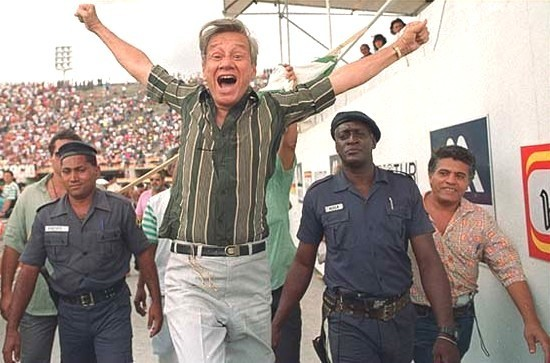
\includegraphics[width=.8\textwidth, height=8cm]{images/bicho07.jpg}
	\caption{Castor de Andrade is shown celebrating after the samba school he sponsored, Mocidade Independente, won the Carnival parade in 1996. He was surrounded by colleagues and police officers. Andrade was the founding president of LIESA (1984--1985) and the wealthiest \emph{bicheiro} of Rio de Janeiro at the time. Source: Folha Imagem. Reproduced in \citet[139]{misse2007illegal}.}
	\label{fig:castor}
\end{figure}

The funding of the samba schools had an indirect effect to the animal game. The patronage also reduced agent-principal problems within the \emph{jogo do bicho}. \emph{Bicheiros} donate to samba school to gather support of the communities, and by doing so they gain access to local information on their business. Clients who have a positive image of the \emph{bicheiro} may denounce fraudsters to their superiors, thus monitoring is cost-effective for animal game managers. Thus, street bookmakers have fewer incentives to cheat. In addition, street sellers are often recruited from the poor communities, so they tend to be immediate beneficiaries of \emph{bicheiros}'s donations \citep{bbc2012aniz}. Hence, funds donated to samba schools and other charities organisations help align the interests of different members of the \emph{jogo do bicho} organisation. The patronage can be interpreted as an illegal version of `profit-sharing', a mechanism which has induced effectively cooperative behaviour in both small and large corporations \citep{cahuc1997profit,fitzroy1987cooperation, kruse1992profit}.

The samba schools have profited from this association too. First, they have gained autonomy from the government. The samba schools do not need to rely exclusively on public funds to organise the parade, and money from the \emph{jogo do bicho} permitted the schools to act independently \citep[209]{chinelli1993vazio}. Second, the support of the \emph{jogo do bicho} has increased the political and social clout of the samba schools. In a country where the state is not present throughout the territory and human right abuses are frequent \citep{ahnen2003,odonnell1993state,pinheiro2000,pinheiro2001}, \emph{jogo do bicho} bankers, and more recently drug traffickers, have provided private governance to poor areas of Rio de Janeiro by enforcing property rights, mediating disputes, and preventing police abuse in the favelas \citep{arias2006dynamics,goldstein2013laughter,leeds1996cocaine}. In return for funds and protection from the \emph{bicheiros}, samba schools have served as intermediaries between the underworld and the political system. Although the \emph{banqueiros} are interested in weak law enforcement against the animal game, politicians have resorted to samba schools to contact \emph{bicheiros} and use their financial and electoral influence in the shanty towns \citep[17]{misse2011crime}. The samba schools, therefore, have increased their bargaining power in the political sphere and extended their reach within Rio's poor communities \citep[215]{chinelli1993vazio}.

\subsection{Political Support}

If politicians were opposed to the \emph{jogo do bicho} in the early twentieth century, their relationship with the animal game bankers have become more ambivalent in the last decades. The collaboration between public authorities and \emph{bicheiros} gained prominence during the military dictatorship (1964--1985) \citetext{\citealp{gaspari2002ditadura}; \citealp{jupiara2015poroes}; \citealp[39]{zaluar2007democratizaccao}}. Given the absence of democratic checks and balances, paramilitaries and police forces colluded to repress potential dissidents of the regime and, frequently, to extort civilians \citep{gorender1999combate,magalhaes1997logica,misse2009acumulaccao,skidmore1990politics}. \emph{Bicheiros} saw the corruption of some members of the military as an opportunity. Wealthy \emph{jogo do bicho} bankers hired rogue police officers not only to work as security guards but to threaten eventual competitors in their regions of influence. The agreement between \emph{bicheiros} and corrupt members of the military was the ultimate responsible for the transformation of the \emph{jogo do bicho} into a `coercive oligopoly' \citep{jupiara2015poroes}. The support of the armed forces meant that new groups would be prohibited from entering the market and that the illegal lottery could operate undisturbed by the government.

The links between \emph{bicheiros} and the public authorities changed after Brazil became a democracy in 1985. In the military regime, government officials were mainly interested in bribes from the animal game. But in the democratic period, votes became a sought-after political resource. \emph{Bicheiros} are important in this sense as they have direct influence over a number of poor communities. Their patronage networks ensure that candidates supported by \emph{bicheiros} receive a substantial amount of votes from areas where campaigning is too difficult or too costly \citep[17]{misse2011crime}.

The Brazilian political system is particularly conductive to clientelistic practices. Brazil has one of the most fragmented party systems in the world, which induces political entrepreneurs to run highly individualised campaigns \citep{figueiredo2000presidential,geddes1992institutional}. In addition, Brazil uses a open-list proportional representation electoral system, that is, each of the 27 states of the federation are considered as at-large electoral districts \citetext{\citealp{ames1995electoral}; \citealp{mainwaring1992brazilian}; \citealp[483]{samuels2000ambition}}. These two elements indicate that Brazilian politicians are often free from the strong requirements of political parties and can run their campaigns with a high degree of independence. Nevertheless, that independence means candidates rely mostly on themselves to raise funds and establish communication with potential voters. Hence, political campaigns in Brazil tend to be expensive and personality-centred.

The support from the \emph{jogo do bicho} mitigates both problems. With respect to the financial costs of campaigns, illegal donations from \emph{bicheiros} help to cover advertising expenses while having the additional benefit of not appearing in the official records of the candidates \citep{congressoemfoco2007bicho,gazetadopovo2007bicho,globo2012bicheiro}. This suggests that \emph{jogo do bicho}-funded politicians can circumvent spending limits and have an electoral advantage over their competitors. As candidates do not know whether their competitors receive funding from the \emph{jogo do bicho} nor the amount each one was paid, their dominant position is to contact the \emph{bicheiros} and join their networks. The situation is a prisoner's dilemma in which candidates would be better off by running cheaper campaigns and not being dependent of \emph{jogo do bicho} bankers, but asymmetric information prevents them from reaching an optimal solution.

\begin{figure}[!htbp]
	\centering
	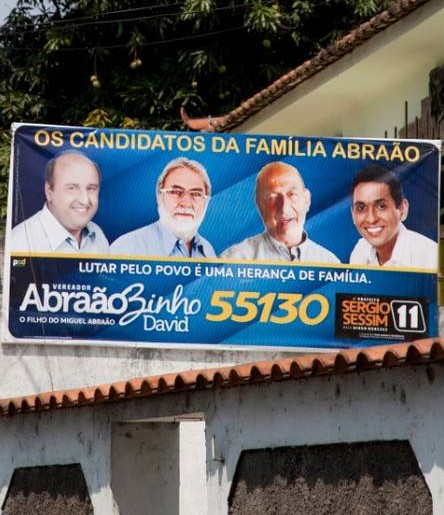
\includegraphics[width=.6\textwidth, height=8cm]{images/bicho08.jpg}
	\caption{Political advertising for Abraãozinho David (right), nephew of the \emph{jogo do bicho} banker Aniz Abraão David (third from left to right). The banner reads: `The Candidates of the Abraão Family: Fighting for the People is a Family Heritage'. Source: \citet{extra2012aniz}.}
	\label{fig:aniz}
\end{figure}

The votes from poor communities are instrumental for aspiring politicians. Brazil has an enforced compulsory voting system; therefore, turnout rates tend to be higher than in other democracies. Consequently, votes have high marginal utility for politicians. As elections may be decided by a small difference, the \emph{bicheiros}' clientelistic ties guarantee a minimum number of votes that politicians can rely upon on election day. Nonetheless, the patronage subverts the preferences of the public and, as such, the democratic process per se. Individuals may be punished if the candidate does not receive the expected number of votes, and are often compelled to vote for politicians that have only loose connections with their communities. Therefore, although voters have the right to choose their representatives, in practice the suffrage is limited for a share of Brazil’s lower classes.

Finally, the \emph{jogo do bicho} patronage highlights a crucial social dilemma within the Brazilian public law. Even though federal judges have prosecuted \emph{bicheiros}, politicians and police forces have no incentives to enforce the punishment. Although Brazilian judges enjoy job stability, the latter groups constantly require local-level support from the \emph{bicheiros}. Politicians and police officers may have accurate information on \emph{jogo do bicho} operations and \emph{bicheiros}' whereabouts, but the federal government cannot rely upon their cooperation. That can be one of the reasons why even after many attempts to arrest \emph{bicheiros}, there has been little progress in that regard in Brazil's latest democratic period (1985--present).

\section{Conclusion}
\label{sec:conclusion}

Past research has shown that criminal organisations face considerable challenges to elicit cooperation from their members and establish close ties with the population \citep[e.g.][]{gambetta1996sicilian,skarbek2011governance,skarbek2012prison,varese2001russian,varese2011mafias}. Yet, the \emph{jogo do bicho} offers a convincing example that it is possible for an illegal syndicate to operate with low levels of violence for more than a hundred years. \emph{Bicheiros} employ a number of strategies to obtain reliable information from their subordinates while offering club goods and other selected benefits to workers. Furthermore, by investing in the Carnival parade \emph{bicheiros} have been able to gather popular and government support. Poor communities have associated with the \emph{bicheiros} to receive welfare provision, whereas politicians have collaborated with them to reap the financial and electoral benefits the \emph{jogo do bicho}'s networks can provide.

Nevertheless, the \emph{jogo do bicho} has also created negative externalities. Violence is used to punish defectors and to constrain competitors. The clientelistic relationship that \emph{bicheiros} have with local politicians have lead to sub-optimal outcomes, such as predatory political campaigning, distortions in electoral representation, and impunity for human rights violations. These negative externalities have long-term effects and still impact the Brazilian public sphere.

Although the \emph{jogo do bicho} has received an increasing attention from scholars, much of its inner workings remain poorly understood. First, the relationship between \emph{bicheiros} and drug dealers is a topic that deserves attention. Brazil has become one of the world's largest consumers of illicit drugs and South America's principal drug trafficking transit route \citep{miraglia2015drugs,misse2011crime}. The question whether \emph{bicheiros} collaborated or opposed the emergent drug dealing business is still unclear. Second, the extent to which \emph{bicheiros} use other businesses, such as hotels or factories, to laundry money has been mentioned by members of the Brazilian judiciary \citep{globo2012bicheiro,globo2015cacaniquel}; however, there is no reliable estimate on its size. Lastly, more research is required to clarify how \emph{bicheiros} from different parts of Brazil coordinate their activities and prevent large-scale conflicts. Cases studies are usually focused on Rio de Janeiro's \emph{bicheiros}, but scholars would benefit from comparative analyses with a larger number of states. This is an important step to elucidate how \emph{bicheiros} continue to influence politics and the public across Brazil.

